\documentclass[convert={density=200}]{standalone}
\usepackage{tikz} 
\usetikzlibrary{arrows}

\begin{document}

 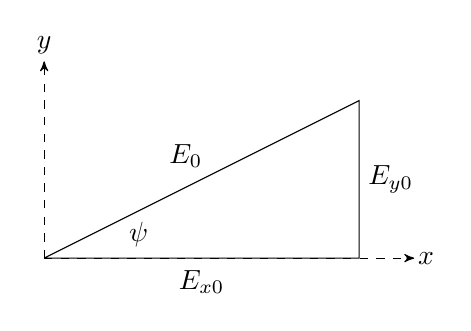
\begin{tikzpicture} [axis/.style={dashed, ->, >=stealth'}, 
 			      pile/.style={thick, ->, >=stealth', shorten <=2pt, shorten >=2pt}]
    \draw (0,0) -- (4,0) -- (4,2) -- (0,0);
    \draw[axis] (0,0) -- (4.7,0);
    \node[] at (4.85,0) {$x$};
    \draw[axis] (0,0) -- (0,2.5);
    \node[] at (0,2.7) {$y$};
    \node[] at (2,-0.3) {$E_{x0}$};
    \node[] at (4.4,1) {$E_{y0}$};
    \node[] at (1.8,1.3) {$E_{0}$};
    \node[] at (1.2,0.3) {$\psi$};
   % \draw[pile] (0,0) -- (1,2);
\end{tikzpicture}

\end{document}